%--------------------------------------------
% Chapter: LINUX OPERATING SYSTEM
%--------------------------------------------
\chapter{Realtime-capable Linux Operating System}
\label{sec:OS}

%- - - - - - - - - - - - - - - - - - - - - - 
% Section: Setting up a bootable SD-Card 
%					 with an Raspbian Distribution
%- - - - - - - - - - - - - - - - - - - - - - 
\section{Creating a bootable SD-Card with a pre-configured Firmware}
\label{sec:OS:sdCardSetup}

For a convenient and easy start with the Raspberry Pi, a pre-configured Raspberry Pi Firmware can be found at the SVN repository folder \texttt{/sys/RPi/}. The pre-configured Firmware Image is based on the EMLID-distribution (see also chapter \ref{sec:OS:emlid}). The EMLID-distribution originates from a open source project\footnote{EMLID-Distribution: \url{http://www.emlid.com/new-raspbian-with-real-time-kernel-jan-2015/}} for a different Raspberry Pi based Quadcopter. It comprises the RT-Kernel patch as well as several optimizations regarding the system configuration to access peripherals that fit to the needs of this project\footnote{The hardware setup as well as the software architecture was planned before the authors have discovered the EMLID-distribution. It was a lucky coincidence, that the EMLID-distribution met almost all core requirements of this project. Because of that, the authors could used the EMLID-distribution as a base distribution during the software development and could develop in parallel - independently from the progress of patching the Raspbian distribution to a RTOS (as shown in chapter \ref{sec:OS:preemptRtPatch}).}.

For this project, pick the archive file \texttt{EMLID\_Preempt\_IP192.168.2.1.zip} from the SVN repository. Unzip the file to get the extracted 8GB Firmware Image.

To write the Firmware Image to a SD Card, use the tool \texttt{Win32DiskImager}\footnote{Download \texttt{Win32DiskImager} at \url{http://sourceforge.net/projects/win32diskimager/}} for Windows based Host machines (as shown in fig. \ref{fig:OS:win32DiskImager}).
\begin{figure}[H]
    \centering
    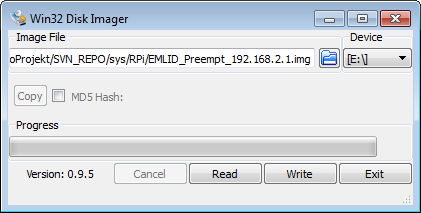
\includegraphics[width=0.65\textwidth]{fig/ch-rt-linux-os/Win32DiskImager}
    \caption[Windows tool Win32DiskImager]{Windows tool Win32DiskImager to write a Raspberry Pi Firmware to a SD Card in a Windows Host System}
    \label{fig:OS:win32DiskImager}
\end{figure}

For Linux based host machines (as well as the Development Environment VM), the built-in program \texttt{dd} can be used to copy the Firmware to a SD card. Therefore, the device handler \texttt{/dev/sd}X has to be determined, first! Issue the command \texttt{lsblk} and search for a disk with the same size as the SD card.\\
Assuming the device handler is \texttt{/dev/sdb} (use device handler of complete disk, without any numbers in the name), the Firmware can be copied with the below shown command.

\textbf{Attention:}\\
A wrong chosen device handler can destroy the operating system of the host machine!
\begin{lstlisting}[language=bash,otherkeywords={unzip,dd,sudo,of}]
cd ../path/to/svnRepository/sys/RPi/
unzip EMLID_Preempt_IP192.168.2.1.zip
sudo dd if=EMLID_Preempt_192.168.2.1.img of=/dev/sdb
\end{lstlisting}

\textbf{Remark:}\\
To use the pre-configured Firmware Image, a SD Card with at least 8GB storage capacity has to be used! Otherwise, the Firmware Image will be too big.

%- - - - - - - - - - - - - - - - - - - - - - 
% Section: Patching Linux Kernel to PREEMPT_RT version
%- - - - - - - - - - - - - - - - - - - - - - 
\section[Building a Real-Time Linux Kernel]{Building a Real-Time Linux Kernel for the Raspberry Pi}
\label{sec:OS:preemptRtPatch}
In the following chapters, the folder structure for the kernel sources and kernel developments on the Development Environment (Virtual Machine) will be evolving such that the following folder structure appears:
\dirtree{%
.1 $\sim$/\DTcomment{Home-directory of the current user}.
.2 rpi\DTcomment{Raspberry Pi related sources and files}.
.3 linux\DTcomment{Linux Kernel sources}.
.3 linux-rt-rpi\DTcomment{EMLID-based Kernel sources (see chapter \ref{sec:OS:emlid})}.
.3 tools\DTcomment{Raspberry Pi toolchain tools}.
}
Therefore, first create the first folder hierarchy \texttt{rpi} with the commands
\begin{lstlisting}[language=bash,otherkeywords={mkdir,cd,dd,sudo}]
cd ~
mkdir rpi
cd rpi
\end{lstlisting}

Next, get latest RT-Kernel patch from the official website of the Linux Kernel Organization, Inc. (\url{https://www.kernel.org/pub/linux/kernel/projects/rt/}). Open the link with a browser in the Development Environment VM and navigate to the current stable release of Linux kernels (version 3.18 at the time of this project). Choose the file \texttt{patch-3.18.XX-rtXX.patch.xz} and copy the URL. Use the copied link to issue the command \texttt{wget} to download the Kernel patch archive into the folder \texttt{$\sim$/rpi/linux}, similar as shown below:
\begin{lstlisting}[language=bash,otherkeywords={mkdir,wget,xcat,dd,sudo}]
cd ~/rpi/
mkdir linux
cd linux
wget https://www.kernel.org/pub/linux/kernel/projects/rt/3.18/patch-3.18.16-rt13.patch.xz
\end{lstlisting}

As the RT-Kernel patch version and the kernel source version \textbf{must match}, the next step will be to get the Linux kernel source according to the latest available RT-patch version.\\
For that purpose, browse to \url{https://github.com/raspberrypi/linux/} to observe the available branches (see fig.\ref{fig:OS:preemptRtPatch:githubBrowser}). After a matching Kernel source branch could be determined, load the Kernel sources to the Development Environment using the command \texttt{git clone [URL]}. With the additional option \texttt{-b}, the corresponding branch can be chosen:
\begin{lstlisting}[language=bash,otherkeywords={cd,dd,sudo}]
cd ~/rpi/
git clone --depth=1 git://github.com/raspberrypi/linux.git -b rpi-3.18.y
\end{lstlisting}

The download of the kernel sources will take some time. According to the available bandwidth of the github servers, this may take even 1 - 2 hours!

\begin{figure}[H]
    \centering
    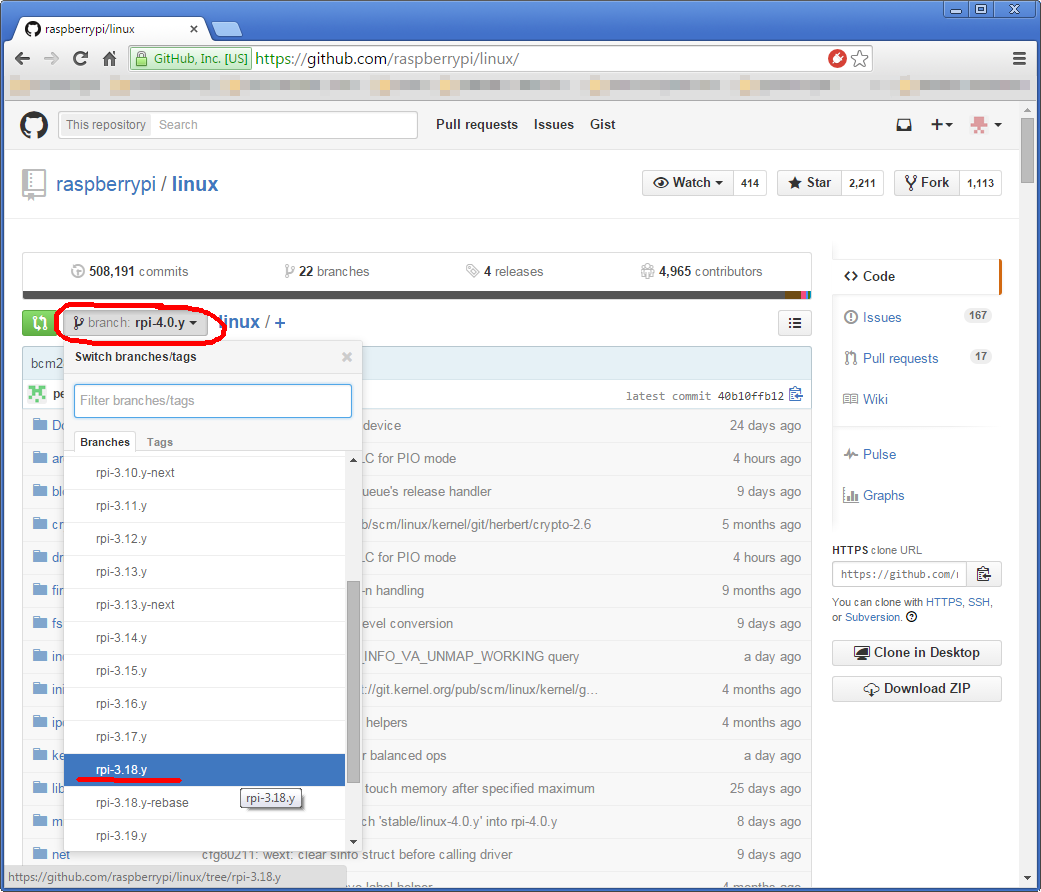
\includegraphics[width=0.85\textwidth]{fig/ch-rt-linux-os/githubBranchesBrowser}
    \caption[Branch list of github's Raspberry Pi Kernel sources]{Branch list of github's repository of the Raspberry Pi's Kernel sources}
    \label{fig:OS:preemptRtPatch:githubBrowser}
\end{figure}

Verify the downloaded kernel version by typing \texttt{make kernelversion} and check that the Kernel version number matches the Kernel version of the RT-Kernel patch.\\
Example:
\begin{lstlisting}[language=bash,otherkeywords={make, xcat,cd,dd,sudo}]
user@ubuntu:~/rpi$ cd linux
user@ubuntu:~/rpi/linux$ make kernelversion
3.18.16
\end{lstlisting}

If the Kernel version numbers match, the RT-Kernel patch can be applied to the Kernel sources. First, a dry run will be executed to check for errors:
\begin{lstlisting}[language=bash,otherkeywords={xcat,cd,dd,sudo}]
cd ~/rpi/linux/
xcat patch-3.18.16-rt13.patch.xz | patch -p 1 --dry-run
\end{lstlisting}

If no errors occur, the patch process can be applied without dry-run option:
\begin{lstlisting}[language=bash,otherkeywords={xcat,dd,sudo}]
xcat patch-3.18.16-rt13.patch.xz | patch -p 1
\end{lstlisting}

Now the Kernel sources have been patched to a Preempt\_RT setup! Next, the Kernel source have to get compiled. Therefore, the Raspberry Pi cross-compile toolchain has to be downloaded, if not already given (see also chapter \ref{sec:sec-VM} for details):
\begin{lstlisting}[language=bash,otherkeywords={dd,sudo}]
cd ~/rpi/
git clone --depth=1 git://github.com/raspberrypi/tools.git
\end{lstlisting}

The following compilation process shown in this documentation is based on the article of \cite{doc:Kern69}. In order to cross-compile the sources in the Development Environment VM, some environment variables in the command line have to be set up:
\begin{lstlisting}[language=bash,otherkeywords={sudo,export}]
export ARCH=arm
export CROSS_COMPILE=../tools/tools/arm-bcm2708/gcc-linaro-arm-linux-gnueabihf-raspbian-x64/bin/arm-linux-gnueabi-
export INSTALL_MOD_PATH=~/rpi/linux/outputLib
mkdir ~/rpi/linux/outputLib
\end{lstlisting}

Now, navigate to the sources and make Raspberry Pi configuration of the kernel sources.
\begin{lstlisting}[language=bash,otherkeywords={make,dd,sudo}]
cd /linux
make bcmrpi_defconfig
\end{lstlisting}

Optionally, with the command \texttt{make menuconfig}, the configuration of the Kernel source setup can be refined. But for the puposes of this project, no adaptions are required.\\
Next, the kernel sources can be cross-compiled, using the command below.

\textbf{Remark:} The option \texttt{-j} defines, how many compilation processes shall be used. Set this value to the same number as CPU cores are available at your machine to achieve the fastest possible cross-compilation.
\begin{lstlisting}[language=bash,otherkeywords={make,dd,sudo}]
make -j4
\end{lstlisting}

\textbf{Attention:}\\
The cross-compilation can take 20minutes up to 2 hours, depending on the resources and CPU power of your development machine! Nevertheless, it is far more efficient to do a cross-compilation than compiling the Kernel sources on the Raspberry Pi directly - this will take 10+ hours!

As a last step of the Kernel compilation, the standard kernel modules have to be linked and installed. According to the environment variables defined above, the kernel modules will be installed at \texttt{$\sim$/rpi/linux/outputLib/}.
\begin{lstlisting}[language=bash,otherkeywords={make,dd,sudo}]
make modules_install
\end{lstlisting}

Get the latest Raspbian distribution at official webpage of the Raspberry Pi Foundation (direct link: \url{http://downloads.raspberrypi.org/raspbian_latest}).\\
Unzip the Firmware Image and copy it to a SD card, according to the steps shown in chapter \ref{sec:OS:sdCardSetup}.

Boot up the device using a keyboard and a display attached to the Raspberry Pi. Log in to the system by using the credentials:
\begin{lstlisting}[language=bash,otherkeywords={make,scp,dd,sudo}]
user: pi
password: raspberry
\end{lstlisting}

Configure the Raspbian distribution to a minimal configuration, issue the command:
\begin{lstlisting}[language=bash,otherkeywords={make,scp,dd,sudo}]
sudo raspi-config
\end{lstlisting}

A graphical user interface will appear as shown in fig. \ref{fig:OS:preemptRtPatch:raspiConfig}. Navigate through the menu, to enable the following options:
\begin{lstlisting}[language=bash,otherkeywords={make,scp,dd,sudo}]
(1) 8 Advanced Options => A4 SSH => <Enable> => <OK>
(2) 8 Advanced Options => A7 I2C => <YES> => <OK> => <YES> => <OK>
(3) 8 Advanced Options => A8 Serial => <NO> => <OK>
(4) 8 Advanced Options => A2 Hostname => <OK> => "HElikopterPi" => <OK>
(5) <FINISH> => <YES>
\end{lstlisting}

\begin{figure}[H]
    \centering
    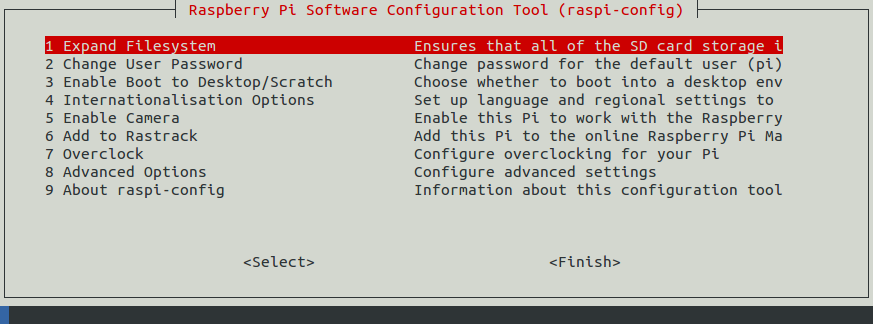
\includegraphics[width=\textwidth]{fig/ch-rt-linux-os/raspiConfig}
    \caption{Graphical configuration tool \texttt{raspi-config} for Raspbian distribution}
    \label{fig:OS:preemptRtPatch:raspiConfig}
\end{figure}

The Raspberry Pi will now reboot to enable all system changes. After the restart, log in again using the keyboard and display attached to the device.

Now, set the network interface to the static network address \texttt{192.168.2.1} by editing the file \texttt{/etc/network/interfaces}:
\begin{lstlisting}[language=bash,otherkeywords={make,scp,dd,sudo,nano}]
sudo nano /etc/network/interfaces
\end{lstlisting}
Ensure that the file is changed such that it matches the excerpt below (assuming your host machine will have the IP \texttt{192.168.2.2}):
\begin{lstlisting}[language=bash,otherkeywords={make,scp,sudo}]
#iface eth0 inet dhcp
iface eth0 inet static
        address 192.168.2.1
        netmask 255.255.255.0
        gateway 192.168.2.2
\end{lstlisting}

As a last step, the root user needs to get a password to enable a comfortable remote file transfer after the Kernel compilation:
\begin{lstlisting}[otherkeywords={make,scp,dd,sudo,su}]
pi@HElikopterPi ~ $ sudo su
root@HElikopterPi:/home/pi# passwd
Enter new UNIX password: 
Retype new UNIX password: 
passwd: password updated successfully
root@HElikopterPi:/home/pi# exit
exit
pi@HElikopterPi ~ $
\end{lstlisting}

Now, the Raspberry Pi can be connected with an Ethernet cable to the Host machine running the Development Environment VM. A ssh connection should be possible with the following command in the Development Machine:
\begin{lstlisting}[language=bash,otherkeywords={make,scp,dd,sudo}]
ssh pi@192.168.22.1
\end{lstlisting}

If the ssh connection could be successfully established, log out and send kernel the compiled Kernel to the Raspbian system by typing the following commands at the Development Environment:
\begin{lstlisting}[language=bash,otherkeywords={make,scp,dd,sudo}]
scp ~/rpi/linux/arch/arm/boot/zImage root@192.168.2.1:/boot/zImage
\end{lstlisting}

Log in at Raspberry Pi with the above state credentials and modify the boot-configuration file \texttt{/boot/config.txt} such that the line \texttt{kernel="zImage"} will be present. If this procedure is done the first time, a easy way to insert the line to the file is the command below:
\begin{lstlisting}[language=bash,otherkeywords={make,scp,dd,sudo}]
sudo su
echo "kernel=zImage" >> /boot/config.txt
exit
\end{lstlisting}

Alternatively, use the text file editor \texttt{nano} to edit \texttt{config.txt}:
\begin{lstlisting}[language=bash,otherkeywords={make,scp,dd,sudo}]
sudo nano config.txt
\end{lstlisting}

Last but not least, copy all kernel modules from the Development Environment VM to the Raspberry Pi using rsync as shown below. Type the following command to the terminal of the Development Environment VM:
\begin{lstlisting}[language=bash,otherkeywords={make,scp,dd,sudo}]
sudo su
rsync -av ~/rpi/linux/outputLib/ root@192.168.2.1:/lib/
exit
\end{lstlisting}

Now the new Kernel and all corresponding Kernel modules are updated. Restart the Raspberry Pi by typing the following command at the Raspberry Pi's command line and wait until the device is up again to reconnection via ssh.
\begin{lstlisting}[language=bash,otherkeywords={make,scp,dd,sudo}]
sudo restart
\end{lstlisting}

After you have logged in, check if the kernel update was successfully. If the new Kernel with the Preempt\_RT patch has been started, the command \texttt{uname -a} should give an output similar as stated below:
\begin{lstlisting}[language=C,otherkeywords={uname,PREEMPT,RT}]
pi@HElikopterPi ~ $ uname -a
Linux HElikopterPi 3.18.14-rt10+ #1 PREEMPT RT Mon Jun 15 21:21:16 CEST 2015 armv6l GNU/Linux
pi@HElikopterPi ~ $
\end{lstlisting}

The relevant parts in the output are highlighted. If the RT-Kernel patch was successfully, the term \texttt{PREEMPT RT} should show up as shown above.

%- - - - - - - - - - - - - - - - - - - - - - 
% Section: Setting up a bootable SD-Card 
%					 with an Raspbian Distribution
%- - - - - - - - - - - - - - - - - - - - - - 
\section[EMLID distribution for development purposes]{Pre-configured EMLID distribution for development purposes}
\label{sec:OS:emlid}

The EMLID-distribution (\url{http://www.emlid.com/}) originates from a open source project\footnote{Download at: \url{http://www.emlid.com/new-raspbian-with-real-time-kernel-jan-2015/}} of an autonomous Raspberry Pi controlled Quadcopter, similar to this project. Different to this project, the EMLID community uses a custom hardware module to extend the hardware capabilities of the Raspberry Pi. In this project, the authors aimed and succeeded to extend the Raspberry Pi with ready-made on market available sensors and boards.

The hardware setup as well as the software architecture of this project was planned before the authors got known about the existence of the EMLID-distribution. It was a lucky coincidence, that the EMLID-distribution meets almost all core requirements of this project. Because of that fact, the authors could use the EMLID-distribution as a base distribution during the software development. In consequence, the software development could be processed in parallel to the other project tasks - especially independently from the progress of patching the Raspbian distribution to a RTOS (applying the RT-Kernel patch as shown in chapter \ref{sec:OS:preemptRtPatch}).

Since some Kernel module driver has been developed during this project, it was also necessary to compile the custom Kernel drivers for the EMLID-distribution. Therefore, get slightly modified Kernel sources of the EMLID-distribution can be found at \url{https://github.com/emlid/linux-rt-rpi}. To download the sources to the Development Environment VM, the following commands can be used:
\begin{lstlisting}[language=bash,otherkeywords={cd,dd,sudo}]
cd ~/rpi/
git clone --depth=1 git://github.com/emlid/linux-rt-rpi.git
\end{lstlisting}

This will download the EMLID Kernel sources that are already modified with an appropriate RT-Kernel patch. All source files will be stored to the directory \texttt{$\sim$/rpi/linux-rt-rpi/}.

In order to compile the EMLID kernel sources, the procedure is identical as shown in chapter \ref{sec:OS:preemptRtPatch} except application of the RT-Kernel patch.

To download the complete EMLID-distribution Firmware, see \url{http://www.emlid.com/new-raspbian-with-real-time-kernel-jan-2015/} or use the pre-configured Firmware of the projects SVN repository at \texttt{/sys/Rpi/}.

%- - - - - - - - - - - - - - - - - - - - - - 
% Section: Configurations of peripherals and busses
%- - - - - - - - - - - - - - - - - - - - - - 
\section{Configurations of peripherals and busses}
\label{sec:OS:configProject}

Due to the specific hardware extension boards and sensors used in this project (see also chapter \ref{sec:hardware:Components}), some minor and basic configurations are needed for a flawless operation of the Raspberry Pi platform.

The following aspects have to be met:
\begin{itemize}
	\item \textbf{UART} port has to be unused (not utilized as kernel debug output) since the GPS receiver of the GPS Hat extension board will occupy the UART channel.
	
	\item \textbf{I2C} bus (Bus No. 1, Bus No. 0 is not used in this part of the project) has to be set to a baudrate of 400kBit/s in order to meet the busload requirements.
	
	\item \textbf{Network} configuration has to be set up (static IP address for the most common development scenario: Raspberry Pi attached via wire to the Development Machine).
\end{itemize}

\subsection*{Network configuration}
Set the network interface to the static network address \texttt{192.168.2.1} by editing the file \texttt{/etc/network/interfaces}:
\begin{lstlisting}[language=bash,otherkeywords={make,scp,dd,sudo,nano}]
sudo nano /etc/network/interfaces
\end{lstlisting}
Ensure that the file is changed such that it matches the excerpt below (assuming your host machine will have the IP \texttt{192.168.2.2}):
\begin{lstlisting}[language=bash,otherkeywords={make,scp,sudo}]
#iface eth0 inet dhcp
iface eth0 inet static
        address 192.168.2.1
        netmask 255.255.255.0
        gateway 192.168.2.2
\end{lstlisting}

Perform the command shown below, to update the network configuration of the Linux Operating System. After the update, the changed network configuration will take place:
\begin{lstlisting}[language=bash,otherkeywords={make,scp,sudo}]
sudo /etc/init.d/networking restart
\end{lstlisting}


\subsection{Raspbian distribution specific}
\label{sec:OS:configProject:raspbian}
To configure the Raspbian distribution such that the \textbf{UART} port can be used by the additional peripherals (GPS receiver) and the \textbf{I2C bus} is activated, issue the following command:
\begin{lstlisting}[language=bash,otherkeywords={make,scp,dd,sudo}]
sudo raspi-config
\end{lstlisting}

A graphical user interface will appear as shown in fig. \ref{fig:OS:configProject:raspbian:raspiConfig}. Navigate through the menu, to enable the following options:
\begin{lstlisting}[language=bash,otherkeywords={make,scp,dd,sudo}]
(1) 8 Advanced Options => A7 I2C => <YES> => <OK> => <YES> => <OK>
(2) 8 Advanced Options => A8 Serial => <NO> => <OK>
(3) <FINISH> => <NO>
\end{lstlisting}

Prevent the Raspberry Pi from rebooting, since the required data rate of the I2C bus has to be configured first.
\begin{figure}[H]
    \centering
    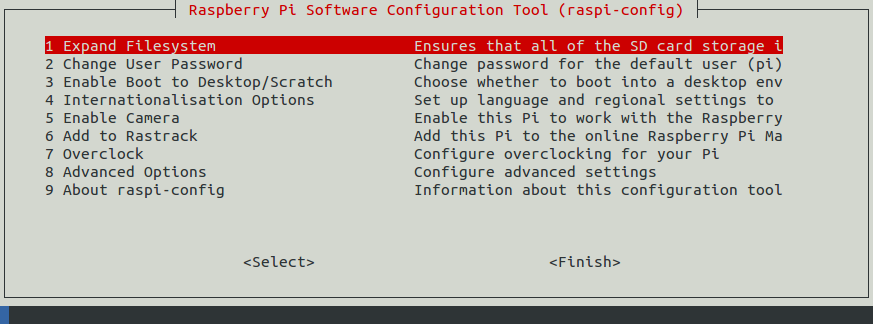
\includegraphics[width=\textwidth]{fig/ch-rt-linux-os/raspiConfig}
    \caption{Graphical configuration tool \texttt{raspi-config} for Raspbian distribution}
    \label{fig:OS:configProject:raspbian:raspiConfig}
\end{figure}
To configure the required \textbf{400kBit/s bauddrate}, navigate to the folder \texttt{/etc/modprobe.d/}. Unlike for the EMLID-distribution, file kernel module configuration file \texttt{i2c.conf} does not exist. To create the file with the proper setup of the I2C bus, perform the following command:
\begin{lstlisting}[language=bash,otherkeywords={make,scp,sudo,nano}]
sudo bash -c "`echo 'options i2c_bcm2708 baudrate=400000' > /etc/modprobe.d/i2c.conf"
\end{lstlisting}

Now reboot the Raspberry Pi so that the configuration changes can take place.

\subsection{EMLID distribution specific}
\label{sec:OS:configProject:emlid}
For the EMLID-distribution, the UART port is configured to the required setup by default. No Kernel debugging messages are put to the serial port. But the default I2C baudrate is set to 1Mhz which is to much. The highest common frequency of the sensors participating on the I2C bus is 400kHz.

\subsection*{I2C configuration}
To specify the required datarate of the I2C bus, navigate to the folder \texttt{/etc/modprobe.d/} and edit the file \texttt{i2c.conf}. Ensure that the content of the file looks like shown below:
\begin{lstlisting}[language=bash,otherkeywords={make,scp,sudo,nano}]
options i2c_bcm2708 baudrate=400000
\end{lstlisting}

Therefore, open \texttt{nano} and edit the file \texttt{i2c.conf}:
\begin{lstlisting}[language=bash,otherkeywords={make,scp,sudo,nano}]
sudo nano /etc/modprobe.d/i2c.conf
\end{lstlisting}